\documentclass{article}
\usepackage[utf8]{inputenc}
\usepackage{listings}
\usepackage{color}
\usepackage[a4paper, margin=1in]{geometry}
\usepackage{url}
\usepackage{fancyvrb}
\usepackage{natbib}
\usepackage{graphicx}
\usepackage[rightcaption]{sidecap}

\definecolor{codegreen}{rgb}{0,0.6,0}
\definecolor{codegray}{rgb}{0.5,0.5,0.5}
\definecolor{codepurple}{rgb}{0.58,0,0.82}
\definecolor{backcolour}{rgb}{0.95,0.95,0.92}

\lstdefinestyle{mystyle}{
    backgroundcolor=\color{backcolour},
    commentstyle=\color{codegreen},
    keywordstyle=\color{magenta},
    numberstyle=\tiny\color{codegray},
    stringstyle=\color{codepurple},
    basicstyle=\footnotesize,
    breakatwhitespace=false,
    breaklines=true,
    captionpos=b,
    keepspaces=true,
    numbers=left,
    numbersep=5pt,
    showspaces=false,
    showstringspaces=false,
    showtabs=false,
    tabsize=2
}

\lstset{style=mystyle}

\title{Ms. Pac-Man AI Assignment}
\author{Jonathan Böcker, Olle Casperson }
\date{October 2016}

%---------------DOCUMENT BEGIN----------------

\begin{document}

\maketitle
%\tableofcontents
%\newpage
\section{Introduction}
In this assignment the objective was to implement an AI controller for Ms. Pacman that is capable of learning from data extracted from previous (human) gameplays. The controller had to be a decision tree
trained by means of an ID3 algorithm\citep{russel2010artifical}. We chose to extend the attribute selection algorithm to C4.5\citep{russel2010artifical}, since it is such a small extension of ID3.

\iffalse  % ------------TVEK-------------------
\begin{itemize}
    \item What input parameters have you used as the input of the decision tree and why?
    \item Why have you discouraged the others?
    \item Did you have to discretize any parameters? Why? How have you accomplished this?
    \item How did you code the learning algorithm and the attribute selection function?
    \item What experiences have you acquired?
\end{itemize}

\section{Ms. Pac-Man}
Ms. Pac-Man is a arcade video game released in the late 1980s. The game is not to be confused with the original Pac-Man game though the gameplay is very similar. It is one of the most popular arcade game of all time and also one of the most successful, selling over 115,000 arcade cabinets.  \citep{mspacmanwiki}

    \subsection{Gameplay}
    The objective is to earn points by eating pills and at the same time avoid the four ghosts that are circling the playing field. It is also possible to eat a larger pill in order to make the ghosts edible and scoring points by eating them. If a ghost, that is not edible, collides with Ms. Pac-Man a life is lost. The game ends when all three lives are lost or when all the levels are completed. To complete a level Ms. Pac-Man must eat all the pills on the playing field.


\fi % ------------------END TVEK----------------------
\section{Input parameters}
\iffalse  % ------------TVEK-------------------
The Ms. Pac-Man implementation that we were given contained some parameters to choose from. For example there are four ghosts on the playing field. Each of the ghosts has attributes like:

\begin{itemize}
     \setlength\itemsep{0em}
    \item Distance (from the ghosts to Ms. Pac-Man)
    \item Direction (in which direction are the ghosts moving in)
    \item Edible (are the ghosts edible)
\end{itemize}

Other parameters that is not concerning the ghosts but still can be used are:

\begin{itemize}
    \setlength\itemsep{0em}
    \item Number of pills left
    \item Number of big pills left
    \item Current game time
    \item Current score
    \item Number of lives left
    \item Ms. Pac-Mans position
    \item Last chosen direction
\end{itemize}
\fi % ------------------END TVEK----------------------

    \subsection{Chosen parameters}
    Our general approach when choosing parameters for the learning algorithm was to look at a human learning to play Ms. Pac-Man. A human player might look at the state of the ghosts, are they edible, close and moving towards Ms. Pac-Man? Based on those criteria the player might have enough information to evade the ghosts and survive a little longer. Our philosophy was to use as little information as possible to solve the task, to avoid overfitting.

    Our biggest issue was to determine, with the recorded data, whether Ms. Pac-Man was facing a ghost at a given time. This seemed impossible and multiple attempts were made to use the last chosen direction and direction of a ghost to make sense of the data. The issue was, when using the last made move as an attribute in any way, the decision tree became extremely shallow. It only required a ghosts direction as an attribute in the root node to determine the next move. This is because the subsets of the data, when finding subsets with an attribute taking a value combined with the class value, all data tuples in the subset has the same class and can be considered as a leaf node when passing that subset to a new node.

    \subsection{Discarded parameters}
    The available parameters are in abundance and parameters such as total time since game started may not be relevant for the survival of Ms. Pac-Man. Similar parameters which does not have any effect to a human players behaviour are ruled out since our guess is that it would not contribute to the heuristic decision tree either.

    \subsection{Discretized parameters}
    Some parameters are continuous, such as distance, and needs to be discretized before used in the decision tree. The reason for this is that the decision tree would have an unreasonable amount of child nodes if there were a child node for each value of a continuous attribute. It needs an unreasonable amount of data to support that many values. This is also why discretizing needs to be reasonable, with not too many possible discrete values.

    The Ms. Pac-Man framework provides a method and enumeration in the \verb|DataTuple| class for this purpose, with seven possible discrete values. We believed this also was too granular and made a similar method and enumeration, limiting the possible values to \verb|HIGH| and \verb|LOW|. The inflection point between these values was chosen to be a normalized distance value of 0.2. This value was simply concluded with guesses and empirical tests to find a moderate value that was good enough.

\section{The learning algorithm}
The learning algorithms main purpose is to create a decision tree that is able to return a \verb|MOVE| when given a game state. Our tree is created when calling a \verb|Node| constructor with the complete dataset and a list of attributes to learn from. This object will be the decision tree root node. It has a \verb|getDecision()| method which will return a \verb|MOVE| object that the learning algorithm views as the most appropriate according to the learning data.

    \subsection{ID3 and C4.5}
    The main part of the learning algorithm is the C4.5 attribute choosing algorithm which, at each node, decides what attribute has the highest benefit when analyzing the set of data given to the node. The data given to the root node is supposedly very impure, since it is recorded from human playthroughs, which probably contains mistakes which lead to the death of Ms. Pac-Man. This means that the information entropy is relatively large and is hard to classify.

    The ID3 algorithm has to find an attribute that leads to a dataset that has the least entropy and highest information gain possible among all attributes. This way the decision tree is guaranteed to be the best tree possible.

    Our class \verb|C45| has only one method visible to outside classes (Listing \ref{attribute}), and one private method (Listing \ref{infod}).

    \SaveVerb{term}|C45.selectAttribute()|
    \begin{lstlisting}[language=Java, caption=Method declaration of \protect\UseVerb{term}, label={attribute}, escapechar=|]
public static String selectAttribute(
            LinkedList<DataTuple> dataList,
            LinkedList<String> attributes) {
    |\dots|
}
    \end{lstlisting}

    \SaveVerb{term2}|C45.calculateInfoD()|
    \begin{lstlisting}[language=Java, caption=Method definition of \protect\UseVerb{term2}, label={infod}, escapechar=|]
private static double calculateInfoD(LinkedList<DataTuple> dataTuples) {
    HashMap<Constants.MOVE, Double> tuplePerClass = new HashMap<>(); |\label{tupleperclass}|
    |\dots|
    // Increase every find by one in the map
    for (DataTuple tuple : dataTuples) {
        tuplePerClass.put(tuple.DirectionChosen,
            tuplePerClass.get(tuple.DirectionChosen) + 1);
    }
    double dataSize = (double) dataTuples.size();
    double infoD = 0;
    for (Constants.MOVE move : Constants.MOVE.values()) { |\label{addingstart}|
        double count = tuplePerClass.get(move);
        if (count > 0) {
            infoD += -(count / dataSize) *
                    (Math.log(count / dataSize) / Math.log(2)); |\label{addingend}|
        }
    }
    return infoD;
}\end{lstlisting}

    Both are static and holds no state between method calls. The \verb|selectAttribute()| method simply returns the name of the most rewarding attribute in a string and the \verb|calculateInfoD()| method returns a \verb|double| value derived of equation \ref{infoD}.
    \begin{equation} \label{infoD}
    Info(D)=-\sum_{i=1}^{m}p_i log_2(p_i)
    \end{equation}

    The variable $p_i$ is simply the number of tuples belonging to a certain class value e.g. \verb|UP| divided with the total number of tuples in the dataset. This is achieved in the code by counting all class value occurrences in a hashmap (Listing \ref{infod}, line \ref{tupleperclass}) and adding $p_i log_2(p_i)$ for every value in the class (Listing \ref{infod}, line \ref{addingstart} - \ref{addingend}) to the \verb|infoD| variable.

    The \verb|selectAttribute()| method loops through all attributes passed to that method and performs a number of operations to find the one with most benefit. It calculates a gain for each attribute according to equation \ref{GainA}:
    \begin{equation} \label{GainA}
    Gain(A)=Info(D)-Info_A (D)
    \end{equation}
    $Info_A (D)$ is explained by equation \ref{InfoAD}:

    \begin{equation} \label{InfoAD}
    Info_A (D)=\sum_{j=1}^{v}\frac{|D_j|}{|D|}\times Info(D_j)
    \end{equation}
    $Gain(A)$ is then used for calulating the gain ratio according to equation \ref{GainRatio}:

    \begin{equation} \label{GainRatio}
    GainRatio(A)=\frac{Gain(A)}{SplitInfo_A (D)}
    \end{equation}
    $SplitInfo_A (D)$ is explained by equation \ref{SplitInfo}:

    \begin{equation} \label{SplitInfo}
    SplitInfo_A (D)=-\sum_{j=1}^{v}\frac{|D_j|}{|D|} \times log_2\bigg( \frac{|D_j|}{|D|}\bigg)
    \end{equation}

    In code, these are implemented as follows in listing \ref{excerptSelect}:

    \begin{lstlisting}[language=Java, caption=Excerpt from \protect\UseVerb{term}, label={excerptSelect}, escapechar=|]
double infoD = calculateInfoD(dataList); |\label{infoDCalc}|
|\dots|
for (String attr : attributes) { |\label{forEveryAttr}|
    |\dots|
    for (String value : Utils.getAttributeVariations(attr)) {
        subset = Utils.createSubset(dataList, field, value); |\label{infoADCalcStart}|
        infoAD += ((double) subset.size() / (double) dataList.size()) *
                                                    calculateInfoD(subset); |\label{infoADCalcEnd}|
        if(subset.size() > 0) {                                             |\label{splitInfoADStart}|
            splitInfoAD += -((double) subset.size() / (double) dataList.size()) *
                    (Math.log((double) subset.size() / (double) dataList.size()) /
                                                            (double) Math.log(2));
        }                                                   |\label{splitInfoADEnd}|
    }
    double gainA = infoD - infoAD; |\label{gainACalc}|
    double gainRatio = Double.MAX_VALUE;          |\label{gainRatioStart}|
    if(splitInfoAD > 0)
        gainRatio = gainA / splitInfoAD;    |\label{gainRatioEnd}|
    |\dots|
}
|\dots|\end{lstlisting}
    First $Info(D)$ on the whole dataset is calculated (Listing \ref{excerptSelect}, line \ref{infoDCalc}), then for every attribute (Listing \ref{excerptSelect}, line \ref{forEveryAttr}) $Info_A (D)$ (Listing \ref{excerptSelect}, line \ref{infoADCalcStart} - \ref{infoADCalcEnd}) and $SplitInfo_A (D)$ (Listing \ref{excerptSelect}, line \ref{splitInfoADStart} - \ref{splitInfoADEnd}) is calculated. $SplitInfo_A (D)$ can only be calculated if the subset ($|D_j|$) is larger than zero, because $log_2 (0)$ is undefined.
    $Gain(A)$ is then calculated (Listing \ref{excerptSelect}, line \ref{gainACalc}) and $GainRatio(A)$ is calculated if $SplitInfo_A (D)$ is greater than zero, otherwise it is set to the biggest possible value  (Listing \ref{excerptSelect}, line \ref{gainRatioStart} - \ref{gainRatioEnd}). This is of course because something cannot be divided by zero, but we assume \(\lim_{SplitInfo_A (D) \to 0}\) which means  \(\lim_{GainRatio(A) \to \infty}\).
    The algorithm then returns the attribute with the highest gain ratio.

    \subsection{The Node class}
    \SaveVerb{node}|Node|
    \begin{SCfigure}[0.5][h]
        \caption{The \protect\UseVerb{node} class diagram}
        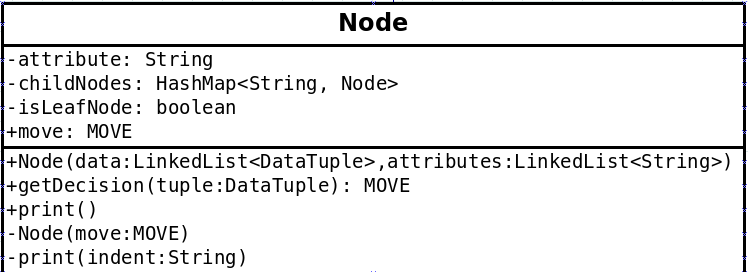
\includegraphics[width=0.6\textwidth]{DiagramNode}
        \label{nodeClassDiag}
    \end{SCfigure}

    The \UseVerb{node} class is both responsible for building the decision tree and being an entity in the resulting decision tree. When using the public constructor, several checks are made to determine if that node is going to be a leaf node or not. First of all, a check is made on the dataset to determine if all datapoints have the same class (Listing \ref{nodepublic}, line \ref{check1}), which qualifies the node as a leaf node.

    Another check is then made to see if there is no attributes left in the attribute list, which if true, sets the node as a leaf node with the majority class in the dataset as the node move (Listing \ref{nodepublic}, line \ref{check2start}-\ref{check2end}).

    \begin{lstlisting}[language=Java, caption=Excerpt from \protect\UseVerb{node} public constructor, label={nodepublic}, escapechar=|]
if (data.size() > 0 && Utils.checkifSetHasSameClass(data)) { |\label{check1}|
    this.move = data.getFirst().DirectionChosen;
    this.isLeafNode = true;
} else if (attributes.size() == 0) {    |\label{check2start}|
    this.move = Utils.findMajorityClass(data);
    this.isLeafNode = true; |\label{check2end}|
} else {
    this.attribute = C45.selectAttribute(data, attributes); |\label{nodeElseStart}|
    attributes.remove(this.attribute);
    for (String value : Utils.getAttributeVariations(this.attribute)) {
        LinkedList<DataTuple> subset = Utils.createSubset(data, attribute, value);
        if (subset.size() > 0) {
            childNodes.put(value, new Node(subset,
                    (LinkedList<String>) attributes.clone()));
        } else {
            childNodes.put(value, new Node(Utils.findMajorityClass(subset)));
        } |\label{nodeElseEnd}|
    }
}
\end{lstlisting}

    If none of those criteria are met, the node will have to ask the C4.5 algorithm for a suitable attribute and produce a child node for each possible value in that attribute (Listing \ref{nodepublic}, line \ref{nodeElseStart}-\ref{nodeElseEnd}). There is a specific case where no subset can be extracted from the original dataset. This is when no datatuples has the sought value in the demanded attribute, in which case the child node has to be a leaf node. Its move will have to be the majority class in the original dataset, and a private constructor is made for those cases, as seen in figure \ref{nodeClassDiag}, page \pageref{nodeClassDiag}.

    After the root node public constructor has finished. the decision tree is done and is ready to make new decisions based on new data. Such decision is retrieved with the \verb|getDecision()| method, which recursively traverse the decision tree to find a leaf node based on the current game state in the \verb|tuple| variable(Listing \ref{getdecmeth}, line \ref{decdef}). The method assumes it is a leaf node until \verb|this.isLeafNode| is evaluated to false (Listing \ref{getdecmeth}, line \ref{leafnodefalse}). If the node is a leaf node it simply returns \verb|this.move|, otherwise it calls one of its child nodes \verb|getDecision()|. Which child node to call is based on the \verb|tuple| string representation of the value sought, stored in the class declared field named the same as \verb|this.attribute|(Listing \ref{getdecmeth}, line \ref{reflect}).

    Not all attributes can be converted to a string representation immediately, e.g. a distance needs to discretized before used as a key in the hashmap(Listing \ref{getdecmeth}, line \ref{distStart}-\ref{distEnd}).

    \SaveVerb{getdec}|getDecision()|
    \begin{lstlisting}[language=Java, caption=The \protect\UseVerb{getdec} method., label={getdecmeth}, escapechar=^]
Constants.MOVE getDecision(DataTuple tuple) { ^\label{decdef}^
    Constants.MOVE returnMove = this.move;
    if (!this.isLeafNode) { ^\label{leafnodefalse}^
        Field field = DataTuple.class.getDeclaredField(this.attribute);^\label{reflect}^
        if (this.attribute.contains("Edible") || this.attribute.contains("Dir")) {
            returnMove = childNodes.get(field.get(tuple).toString()).getDecision(tuple);
        } else if (this.attribute.contains("Dist")) { ^\label{distStart}^
            returnMove = childNodes.get(
                    Utils.discretizeDistance((Integer) field.get(tuple)).toString()
            ).getDecision(tuple);  ^\label{distEnd}^
        } else System.out.println("This shouldn't happen. Kick the author in the butt");
    }
    return returnMove;
}\end{lstlisting}

\section{Accuracy of the classifier}
Listing \ref{verifycode} shows the method for verifying the accuracy of the classifier. The method receives the data that the AI-controller has been trained with and compares every chosen direction with the data. For every tuple whose move matches the training data, \verb|correctGuesses| increases. By dividing the \verb|correctGuesses| by the size of the list containing training data we can get the classifiers accuracy in percentage. The result is then printed to the console.

    \SaveVerb{verify}|verifyData()|
    \begin{lstlisting}[language=Java, caption=The \protect\UseVerb{verify} method, label={verifycode}, escapechar=|]
private void verifyData(LinkedList<DataTuple> dataList) {
	int correctGuesses = 0;
	for (DataTuple tuple : dataList)
		if (tuple.DirectionChosen.equals(this.rootNode.getDecision(tuple)))
			correctGuesses++;

	System.out.println("\n>> Classifier accuracy: " +
	            correctGuesses / (double)dataList.size());
} \end{lstlisting}

\section{Conclusions}
There are of course several approaches that could have been taken to the different subproblems of this assignment. Some requirements was mentioned in the specification but in most cases it didn't specify exactly with what means and methods the requirements should be filled. For example other parameters could have been chosen for the AI-controller to make its decision from. Though we already have elaborated our method of choosing parameters previously in this report it should be mentioned that other ways could have been better. Maybe other parameters, in combination, would make a better AI-player.

\bibliographystyle{plain}
\bibliography{references}
\end{document}
